\documentclass[border=4pt]{standalone}

\usepackage{tikz}

\definecolor{otblue}{HTML}{0072B2}
\definecolor{otorange}{HTML}{E69F00}
\definecolor{otteal}{HTML}{009E73}
\definecolor{otpurple}{HTML}{CC79A7}
\definecolor{otgray}{HTML}{5A5A5A}

\begin{document}
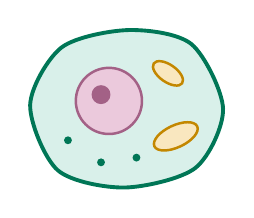
\begin{tikzpicture}[line width=0.9pt]
  \filldraw[draw=otteal!75!black, fill=otteal!15, line width=1.4pt] plot[smooth cycle] coordinates {(1.25,0) (0.85,0.82) (0.05,1) (-0.8,0.78) (-1.2,0.05) (-0.85,-0.78) (0,-1) (0.9,-0.75)};
  \filldraw[draw=otpurple!80!black, fill=otpurple!40] (-0.2,0.1) circle[radius=0.42];
  \fill[otpurple!80!black] (-0.3,0.18) circle[radius=0.12];
  \filldraw[draw=otorange!85!black, fill=otorange!25, rotate around={25:(0.65,-0.35)}] (0.65,-0.35) ellipse[x radius=0.3, y radius=0.14];
  \filldraw[draw=otorange!85!black, fill=otorange!25, rotate around={-35:(0.55,0.45)}] (0.55,0.45) ellipse[x radius=0.22, y radius=0.11];
  \foreach \x/\y in {-0.72/-0.4,-0.3/-0.68,0.15/-0.62}{\fill[otteal!75!black] (\x,\y) circle[radius=0.05];}
\end{tikzpicture}
\end{document}
